\chapter{Congruencia biológica}
Esperamos que los conocimientos (entendidos como nociones de similitud) de los distintos espacios (el de expresión y el biológico) sean diferentes pero no ortogonales. Por lo tanto, una vez detectadas las estructuras en distintas resoluciones en el espacio de expresión, nos interesará cuantificar la congruencia biológica de las mismas. Para ello haremos uso de varios índices, BHI, $BHI_{IC}$, $BHI_{Resnik}$, zBHI e ID que servirán como criterios biológicos de validación externos.

\section{Índice de homogeneidad biológica}
El índice de homogeneidad biológica (o BHI por sus siglas en inglés) de una partición, introducido por Datta \cite{Datta2006} es un observable que cuantifica el grado en que una partición presenta grupos biológicamente homogéneos, reportando, para cada grupo, la máxima proporción de pares de genes agrupados que comparten una misma clase funcional de Ontología Génica. Consideremos dos genes $x$ e $y$ que pertenecen a un mismo grupo $D$ de una partición dada, con un total de $k$ grupos, y sean $C(x)$ y $C(y)$ los conjuntos de todas las clases funcionales que tienen anotados a los genes $x$ e $y$ respectivamente. Sea además la función indicadora $I(C(x)=C(y))$ que toma el valor $1$ si hay al menos una clase en donde ambos genes estén anotados, y $0$ en caso contrario. Entonces, el índice de homogeneidad biológica queda definido como:
\begin{equation}
	BHI = \frac{1}{k}\sum\limits_{j=1}^k\frac{1}{n_j(n_j-1)}\sum\limits_{x\neq y\in D_j}I(C(x)=C(y))
\end{equation}
con $n_j$ la cantidad de genes anotados en el grupo $D_j$.\\

\subsection{Modificaciones al Índice de homogeneidad biológica}
Presentaremos a continuación dos variantes del BHI que modificarán la función indicadora para hacer uso de la similaridad semántica y del contenido de información génico.\\
El índice de homogeneidad biológica con contenido de información ($BHI_{IC}$) para un grupo se define como:
\begin{equation}
	BHI_{IC} = \frac{1}{k}\sum\limits_{j=1}^k\frac{1}{n_j(n_j-1)}\sum\limits_{x\neq y\in D_j}I(C(x)=C(y))IC(Gx)
\end{equation}
donde el $IC(Gx)$ es el contenido de información del gen $x$, definido como el máximo de los contenidos de información de los conceptos en los que el gen $x$ se encuentra anotado.\\
Este índice permite pesar la homogeneidad biológica de un grupo la especificidad de los genes que lo componen.\\
Por otro lado, el índice de homogeneidad biológica Resnik para un grupo, $BHI_{Resnik}$ queda definido como:
\begin{equation}
	BHI_{Resnik} = \frac{1}{k}\sum\limits_{j=1}^k\frac{1}{n_j(n_j-1)}\sum\limits_{x\neq y\in D_j}I(C(x)=C(y))Sim_{rcmax}(C(x), C(y))
\end{equation}
donde $Sim_{rcmax}(C(x), C(y))$ es como fuera definida en \ref{eq:sim_rcmax}.\\
Este índice pesa la homogeneidad biológica de un grupo por la similaridad semántica de los genes que lo componen. Notar que en $BHI_{IC}$ el peso viene dado por la especificidad de cada gen individual que compone una partición, mientras que en $BHI_{Resnik}$ el peso está dado por la similaridad semántica entre pares de genes.\\
Finalmente, el índice de homogeneidad biológica estandarizado para un grupo, zBHI, se define como:
\begin{equation}
	zBHI = \frac{BHI-<BHI_r>}{s(BHI_r)}
\end{equation}
donde $<BHI_r>$ es el valor medio del conjunto de valores del BHI del grupo para un control nulo de 1000 reasignaciones de las etiquetas de la partición y $s(BHI_r)$ es la desviación estandar de la muestra para el mismo conjunto.\\
Se realizó además dos tipos de controles nulos.\\
El primero, un control nulo que llamaremos ``control nulo 1'', se realizó tomando de entre todos los tratamientos 6000 genes que pasaron los filtros. Se formaron grupos de distinto tamaño, desde grupos de 2 genes hasta grupos de \hl{500} genes tomando genes al azar de entre los 6000 con reposición. Para cada tamaño, se realizaron 1000 grupos aleatorios y se calculó su BHI. Se encontró que el valor medio de los ensambles se mantenía aproximadamente constante, mientras que existía una dependencia de la desviación estandar con el tamaño de los grupos. Se realizaron dos ajustes por funciones de ley de potencias, para tamaños entre 1 y 50 y de 51 en adelante. Las funciones halladas permiten rápidamente obtener el BHI aleatorio medio para una partición de cualquier tamaño y su desviación estandar.\\
El segundo, que llamaremos ``control nulo 2'', consistió en realizar 1000 reasignaciones aleatorias de las etiquetas de cada partición y calcular el BHI de cada grupo de la misma. Encontramos que la media de BHI calculada de esta manera coincidía con la del control nulo anterior, pero no así su desviación estandar. Concluimos que la diferencia fundamental se basa en que en el segundo caso, en la reasignación de etiquetas, se mantiene siempre la estructura de tamaños de la partición, mientras que en el primer caso, cada grupo fue tomado por separado.\\
Para caracterizar el comportamiento de cada uno de estos índices se midieron los mismos para cada tratamiento y se calculó su correlación de a pares de índices. La figura \ref{fig:correlacion_de_a_pares_bhi} muestra las distribuciones y correlaciones de a pares para estos índices en el tratamiento ``Frío''. Se encuentra que los índices modificados tienen una alta correlación entre ellos y con BHI, y por lo tanto, no aportan más información que la que se obtiene a través del índice original. Por ser el más sencillo de calcular, es el que utilizaremos como criterio de validación externa de la calidad de una partición.
\begin{figure}[h]
    \centering
    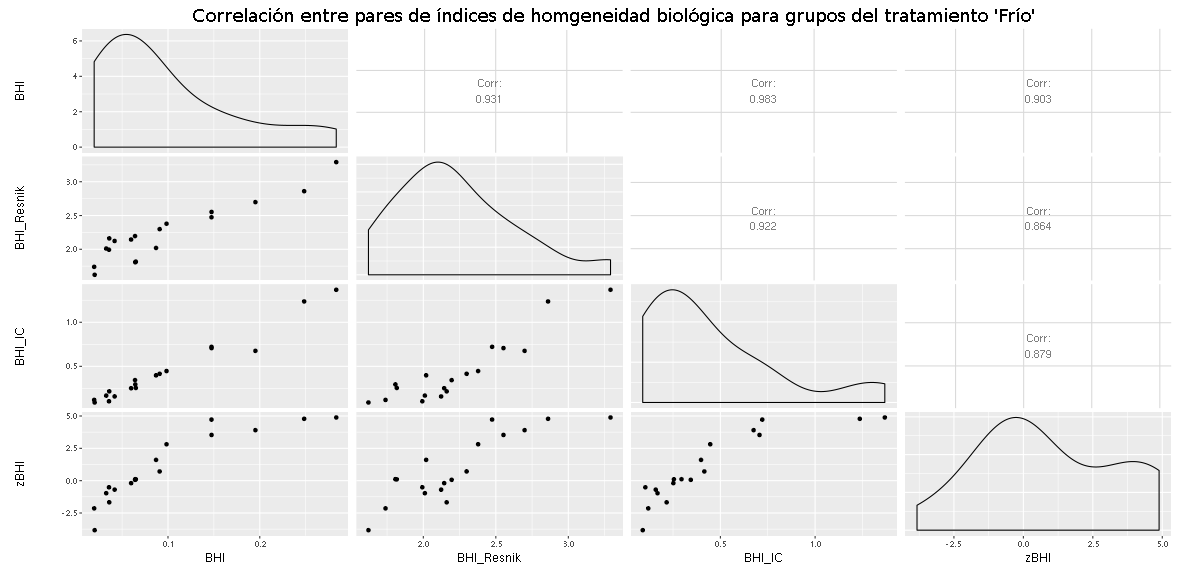
\includegraphics[width=0.8\textwidth]{correlacion_de_a_pares_bhi}
    \caption{Correlación de a pares para los distintos índices de homogeneidad biológica presentados para cada uno de los grupos del tratamiento 'Frío' obtenidos con $ds=1$. Se observa que todos los índices tienen una alta correlación entre si.}
    \label{fig:correlacion_de_a_pares_bhi}
\end{figure}

\section{Densidades de interacción}
El índice de Densidades de interacción, o ID, de una partición, introducido por Dutkowski en \cite{Dutkowski2013} es un observable que cuantifica el grado en que los genes de una partición comparten anotaciones en GO y además forman parte del mismo grupo. El mismo se define para una ontología GO (utilizaremos las definidas en la sección \label{sec:go}, GO BPA, GO BPB y GO CC) y una partición como:
\begin{equation}
	ID(GO_j) = \frac{# Pares de genes en GO_j que aparecen juntos en un mismo grupo C_x}{# Pares de genes en GO_j}
\end{equation}
Por ejemplo, si 

\section{Congruencia biológica de las particiones}

Los valores de BHI calculados para cada uno de los grupos del tratamiento ``frío'' en las particiones k-means (puntos rojos), $ds1$ (triángulos verdes) y $ds4$ (cuadrados azules) se presentan en las figuras \ref{fig:bhi_km_ds1_ds4_control1}, con control nulo 1 y \ref{fig:bhi_km_ds1_ds4_control2} con control nulo 2. Los grupos fueron ordenados según su masa de forma creciente.\\
Se observa que de los dos grupos de kmeans, solo uno presenta un BHI superior a una desviación estandar para el control nulo 1 y del tercer cuartil para el control nulo 2, mientras que para $ds1$, el 45\% de los grupos superan una desviación estandar para control nulo 1 y el 30\% de los grupos superan el tercer cuartil para el control nulo 2.
\begin{figure*}[t!]
    \centering
    \begin{subfigure}[t]{0.8\textwidth}
    \centering
    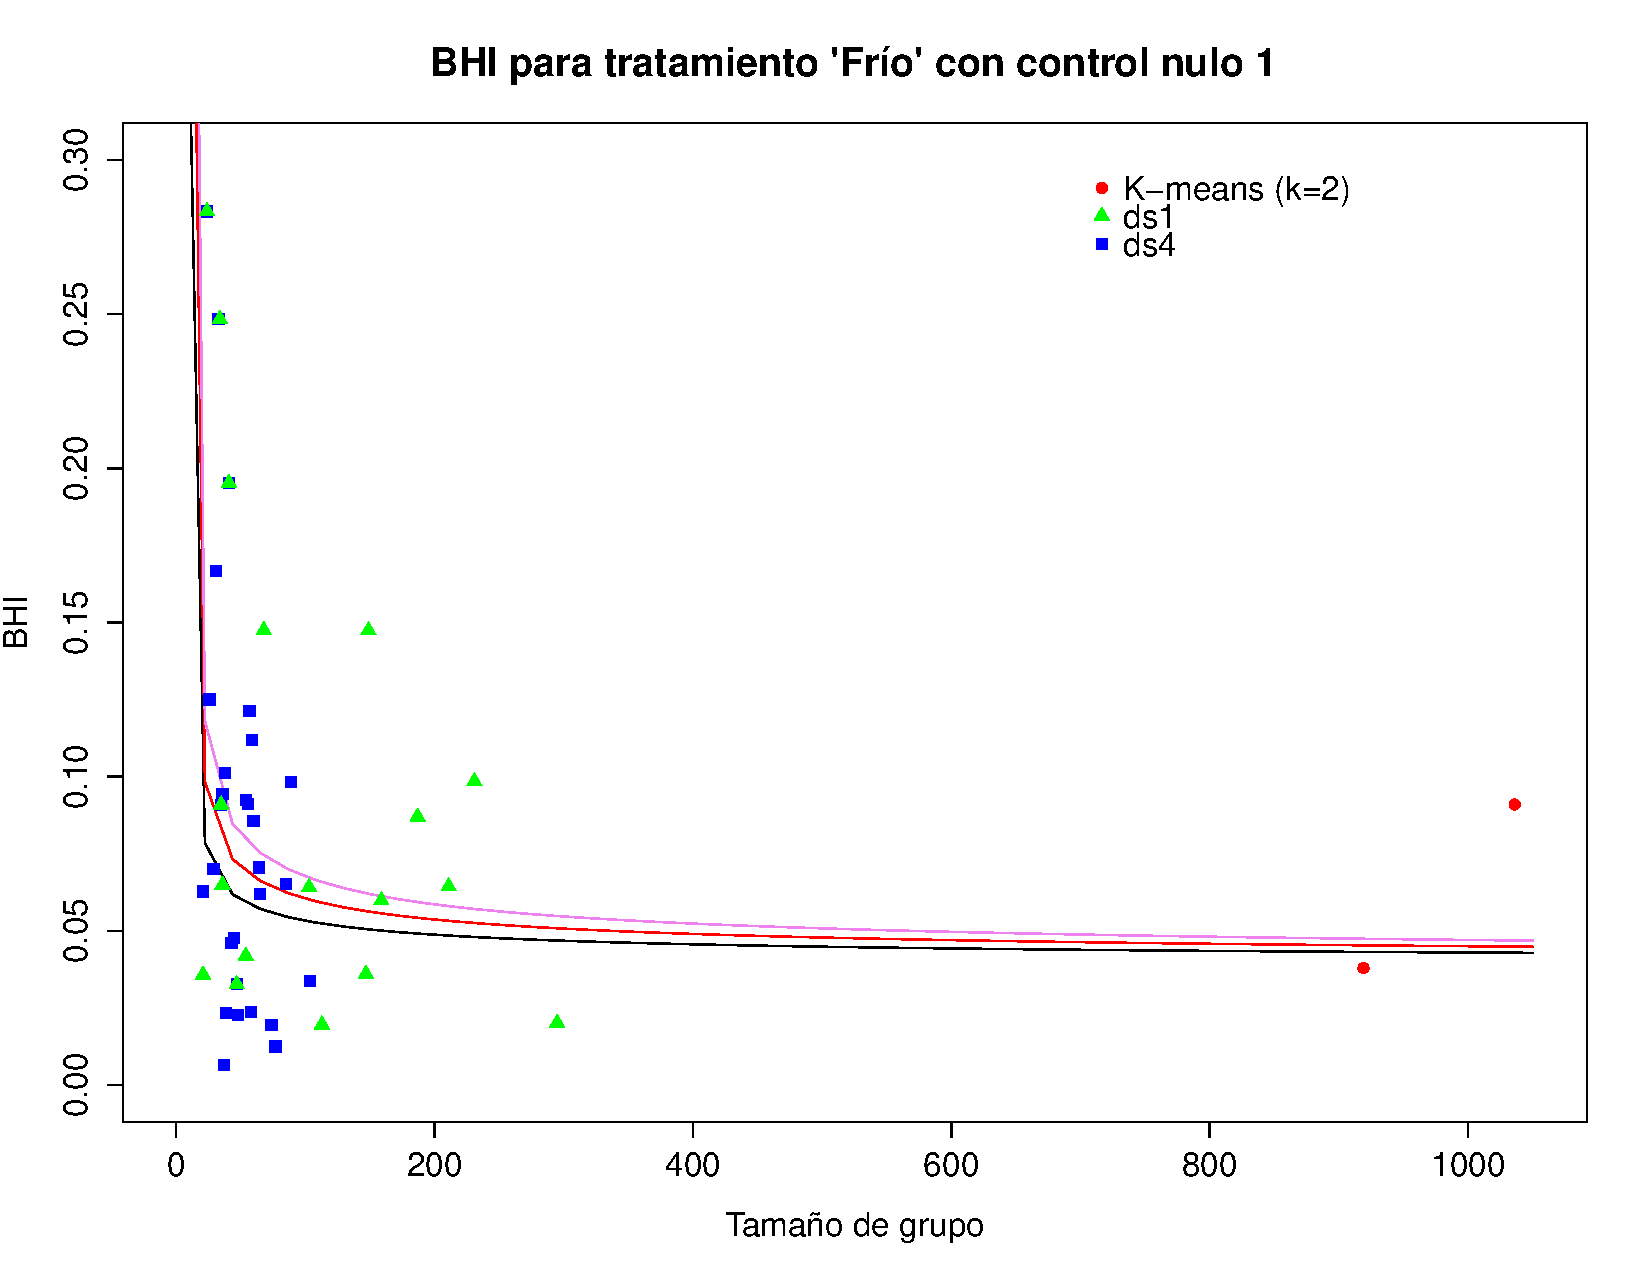
\includegraphics[width=1\textwidth]{bhi_km_ds1_ds4_control1}
    \caption{BHI para cada uno de los grupos del tratamiento 'Frío' obtenidos con kmeans, $ds1$ y $ds4$ y control nulo 1. En turquesa, el valor medio del BHI, en violeta una desviación estandar por sobre el valor medio y en negro una desviación estandar por debajo del mismo.}
    \label{fig:bhi_km_ds1_ds4_control1}
    \end{subfigure}
    \begin{subfigure}[t]{0.8\textwidth}
    \centering
    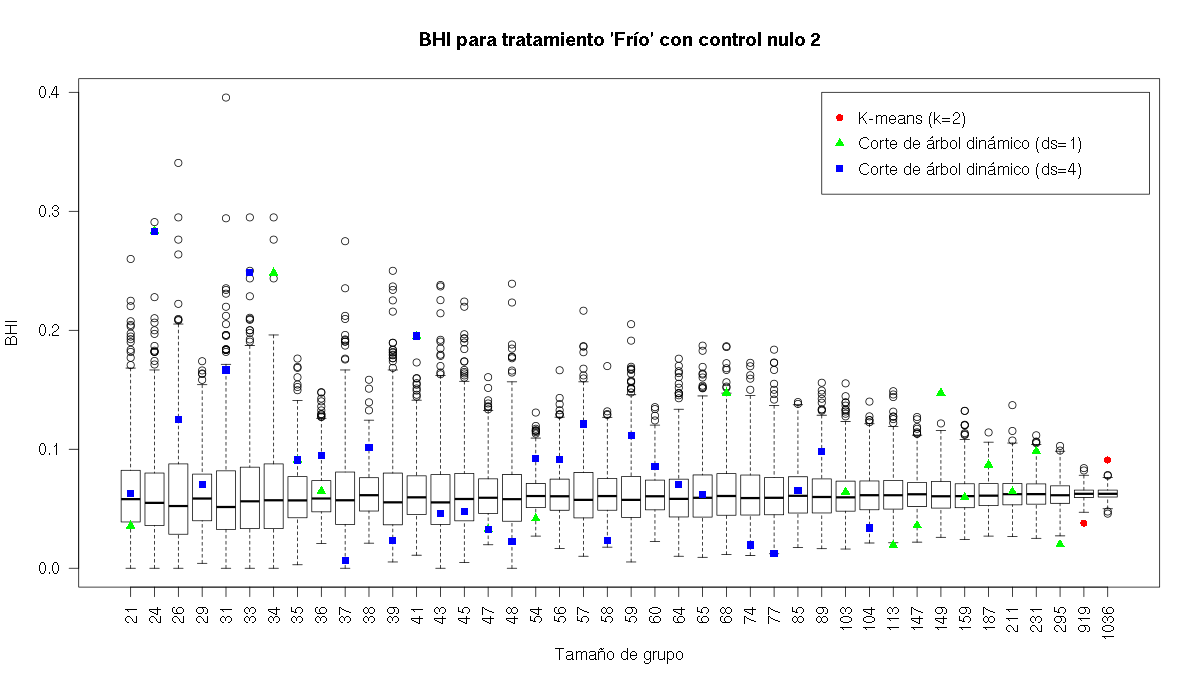
\includegraphics[width=1\textwidth]{bhi_km_ds1_ds4_control2}
    \caption{BHI para cada uno de los grupos del tratamiento 'Frío' obtenidos con kmeans, $ds1$ y $ds4$, y control nulo 2.}
    \label{fig:bhi_km_ds1_ds4_control2}
    \end{subfigure}
    \caption{Índice de Homogeneidad Biológica, BHI, para cada uno de los grupos del tratamiento 'Frío' obtenidos con kmeans, $ds1$ y $ds4$ y controles nulos.}
\end{figure*}

Finalmente, para la partición $ds4$, aproximadamente el 40\% de los grupos presenta un BHI por sobre una desviación estandar para el control nulo 1 y un 50\% presenta un BHI por sobre el tercer cuartil del control nulo 2. 

Esta baja calidad en el índice BHI de las particiones se encontró de forma similar a lo largo de todos los tratamientos. Esto sugiere que si bien el aumentar la granularidad de la partición con el método corte de árbol dinámico resulta en un aumento de la consistencia biológica global de las estructuras observadas, esto no implica que las resoluciones utilizadas sean las óptimas, ya que por lo general el BHI no es superior al del control nulo.\\
A pesar de que en el análisis de estructura de los grupos obtenidos por medio de los métodos k-means, $ds1$ y $ds4$ encontramos que todos los métodos producen particiones altamente coherentes, el análisis de BHI indica que las particiones halladas no pueden ser fácilmente interpretadas a la luz del conocimiento biológico almacenado en GO.